% UTF-8 encoding
% Compile with latex+dvipdfmx, pdflatex, xelatex or lualatex

\documentclass[hyperref, UTF8]{ctexart}
\usepackage{amssymb}
\usepackage{amsmath}
\usepackage{graphicx}
\usepackage{subfigure}
\usepackage{geometry}
\usepackage{caption}
\usepackage{upgreek}
\newcommand{\under}[1]{\frac{1}{#1}}
\newcommand{\underpone}[1]{\frac{#1}{1+#1}}
\newcommand{\volt}{{\rm V}}
\newcommand{\source}{{\rm S}}
\newcommand{\second}{{\rm s}}
\newcommand{\radian}{{\rm rad}}
\newcommand{\ampere}{{\rm A}}
\newcommand{\milliampere}{{\rm mA}}
\newcommand{\microampere}{{\rm \upmu A}}
\newcommand{\hertz}{{\rm Hz}}
\newcommand{\kilohertz}{{\rm kHz}}
\newcommand{\megahertz}{{\rm MHz}}
\newcommand{\ohm}{\Omega}
\newcommand{\kiloohm}{{\rm k}\Omega}
\newcommand{\watt}{{\rm W}}
\newcommand{\kilowatt}{{\rm kW}}
\newcommand{\degree}{^{\circ}}
\newcommand{\farad}{{\rm F}}
\newcommand{\microfarad}{{\rm \upmu F}}
\newcommand{\millifarad}{{\rm mF}}
\newcommand{\henry}{{\rm H}}
\newcommand{\J}{{\rm j}}
\newcommand{\D}{{\rm d}}
\newcommand{\E}{{\rm e}}
\newcommand{\CMRR}{{\rm CMRR}}

\title{电子学基础——第十次作业}
\author{LXQ}
\date{2019.12.12}

\geometry{left=2.0cm, right=2.0cm, top=2.5cm, bottom=2.5cm}
\linespread{1}

\begin{document}

\maketitle
\paragraph{8.10} \label{8.10}
    A truck weighing station inorporates a sensor whose resistance varies linearly with the weight: $R_S = R_0 + \alpha W$. Here $R_0$ is a constant value, $\alpha$ a proportionality factor, and $W$ the weight of each truck. Suppose $R_S$ plays the role of $R_2$ in the noninverting amplifier (Fig. 8-47). Also, $V_{in} = 1 \volt$. Determine the gain of the system, defined as the change in $V_{out}$ divided by the change in $W$. 

    \begin{figure}[!htb]
        \centering
        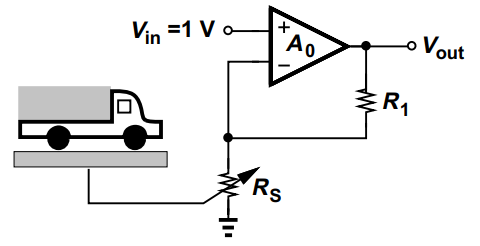
\includegraphics[width=0.320\textwidth]{p8-47.png}
        \caption*{Figure 8-47}
    \end{figure}

\paragraph{解}
    $$V_- = V_+ = 1\volt$$
    $$\therefore V_{out} = V_+ + \frac{V_-}{R_S}\cdot R_1 = (1+\frac{R_1}{R_S})V_{in}$$
    $$\therefore V_{out} = (1+\frac{R_1}{R_0 + \alpha W})V_{in}$$
    $$\therefore \frac{\partial V_{out}}{\partial W} = \frac{-\alpha R_1 V_{in}}{(R_0+\alpha W)^2} = \frac{-\alpha R_1}{(R_0+\alpha W)^2}$$

\paragraph{8.17} \label{8.17}
    An inverting amplifier is designed for a nominal gain of $8$ and a gain error of $0.1\%$ using an op amp that exhibits an output impedance of $2\kiloohm$. If the input impedance of the circuit must be equal to approximately $1\kiloohm$, calculate the required open-loop gain of the op amp.

\paragraph{解}
    \begin{gather*}\left\{\begin{aligned}
        \frac{R_F}{R_{in}} & = 8 \\
        \frac{1}{A_0}(1+\frac{R_F}{R_{in}}) & = 0.1 \%
    \end{aligned}\right.\end{gather*}
    $$\therefore A_0 = 9000$$

\paragraph{8.19} \label{8.19}
    The integrator of Fig. 8-51 senses an input signal given by $V_{in}=V_0\sin \omega t$. Determine the output signal amplitude if $A_0=\infty$. 

    \begin{figure}[!htb]
        \centering
        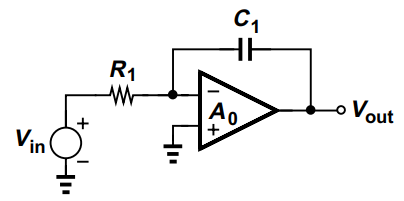
\includegraphics[width=0.269\textwidth]{p8-51.png}
        \caption*{Figure 8-51}
    \end{figure}        

\paragraph{解}
    $$\dot V_{out} = - \frac{\J}{\omega C_1 R_1} \dot V_{in}$$
    则$V_{out}$振幅为$\frac{V_0}{\omega C_1 R_1}$

\paragraph{8.24} \label{8.24}
    The differentiator of Fig. 8-52 is used to amplify a sinusodial input at a frequency of $1\megahertz$ by a factor of $5$. If $A_0 = \infty$, determine the value of $R_1C_1$.

    \begin{figure}[!htb]
        \centering
        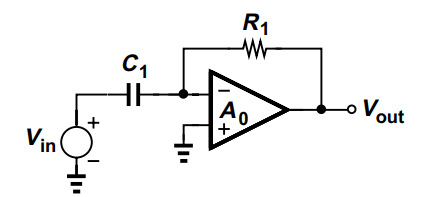
\includegraphics[width=0.283\textwidth]{p8-52.png}
        \caption*{Figure 8-52}
    \end{figure}

\paragraph{解}
    $$\dot V_{out} = \J R_1 C_1 \omega \dot V_{in}$$
    $$\therefore R_1 C_1 \omega = 5, R_1 C_1 = 7.96 \times 10^{-7} \second/\radian^{-1}$$

\paragraph{8.32} \label{8.32}
    The voltage adder of Fig. 8-54 employs and op amp having a finite output impedance. $R_{out}$. Using the op amp model depicted in Fig. 8-44, compute $V_{out}$ in terms of $V_1$ and $V_2$.

    \begin{figure}[!htb]
        \centering
        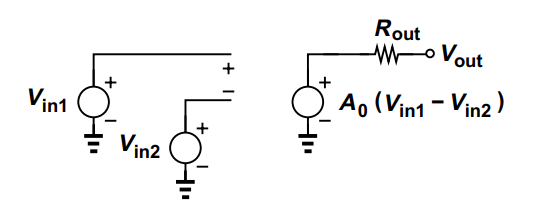
\includegraphics[width=0.365\textwidth]{p8-44.png}
        \caption*{Figure 8-44}
    \end{figure}
    \begin{figure}[!htb]
        \centering
        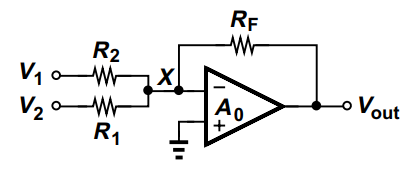
\includegraphics[width=0.278\textwidth]{p8-54.png}
        \caption*{Figure 8-54}
    \end{figure}        
        
\paragraph{解}  
    等效电路如图 p8-32 所示。

    \begin{figure}[!htb]
        \centering
        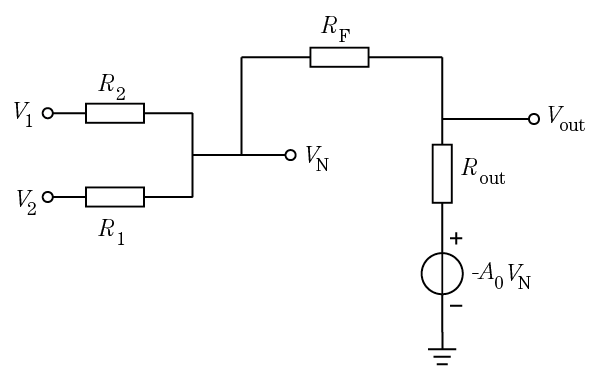
\includegraphics[width=0.407\textwidth]{p8-32-sol.png}
        \caption*{Figure p8-32}
    \end{figure}

    \begin{gather*}\left\{\begin{aligned}
        V_{out} & = V_N - R_F\left(\frac{V_1-V_N}{R_2}+\frac{V_2-V_N}{R_1}\right) \\
        \frac{V_N + A_0 V_N}{R_F + R_{out}} &= \frac{V_1-V_N}{R_2}+\frac{V_2-V_N}{R_1}
    \end{aligned}\right.\end{gather*}
    $$\therefore V_{out} = \frac{(R_1V_1+R_2V_2)\left[1-\frac{R_F(1+A_0)}{R_F+R_{out}}\right]}{R_1 + R_2 + \frac{R_1R_2(1+A_0)}{R_F+R_{out}}}$$

\paragraph{8.33} \label{8.33}
    Due to a manufacturing error, a parasitic resistance $R_P$ has appeared in the adder of Fig. 8-55. Calculate $V_{out}$ in terms of $V_1$ and $V_2$ for $A_0 = \infty$ and $A_0 < \infty$. (Note that $R_P$ can also represent the input impedance of the op amp.)

    \begin{figure}[!htb]
        \centering
        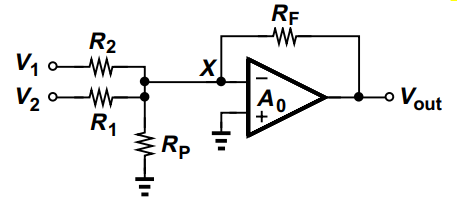
\includegraphics[width=0.305\textwidth]{p8-55.png}
        \caption*{Figure 8-55}
    \end{figure}
        
\paragraph{解}
    等效电路如图 p8-33 所示。

    \begin{figure}[!htb]
        \centering
        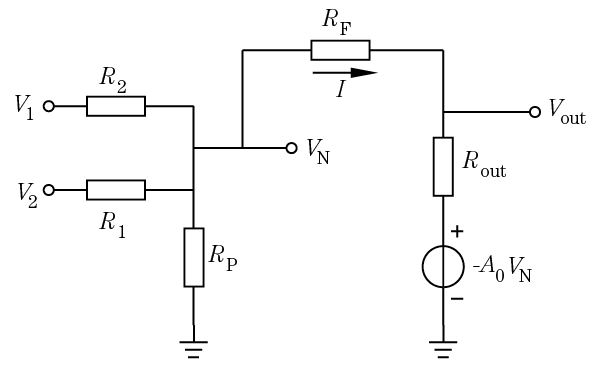
\includegraphics[width=0.405\textwidth]{p8-33-sol.png}
        \caption*{Figure p8-33}
    \end{figure}
        
    \begin{gather*}\left\{\begin{aligned}
        I & = \frac{V_N + A_0 V_N}{R_F + R_{out}} \\
        I & = \frac{V_1 - V_N}{R_2} + \frac{V_2-V_N}{R_1} - \frac{V_N}{R_P} \\
        V_{out} & = V_N - R_F I
    \end{aligned}\right.\end{gather*}
    $$\therefore V_{out} = \left[1-\frac{R_F(1+A_0)}{R_F+R_{out}}\right]\frac{\frac{V_1}{R_2} + \frac{V_2}{R_1}}{\under{R_2} + \under{R_1} + \under{R_P} + \frac{1+A_0}{R_F + R_{out}}}$$
    $$R_{out} \rightarrow +\infty, V_{out} \rightarrow \frac{\frac{V_1}{R_2} + \frac{V_2}{R_1}}{\under{R_2} + \under{R_1} + \under{R_P}}$$

\paragraph{8.34} \label{8.34}
    Consider the voltage adder illustrated in Fig. 8-56, where $R_P$ is a parasitic resistance and the op amp exhibits a finite input inpedance. With the aid of the op amp model shown in Fig. 8-44, determine $V_{out}$ in terms of $V_1$ and $V_2$.

    \begin{figure}[!htb]
        \centering
        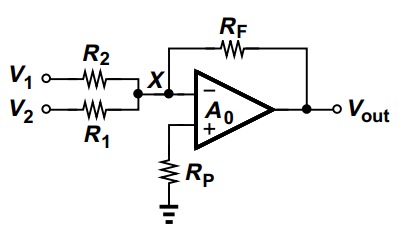
\includegraphics[width=0.271\textwidth]{p8-56.png}
        \caption*{Figure 8-56}
    \end{figure}

\paragraph{解}
    等效电路如图 p8-34 所示。由于$V_P$处无电流,则$V_P=0$,从而可以忽略$R_P$的影响,则答案同题 8.32:

    \begin{figure}[!htb]
        \centering
        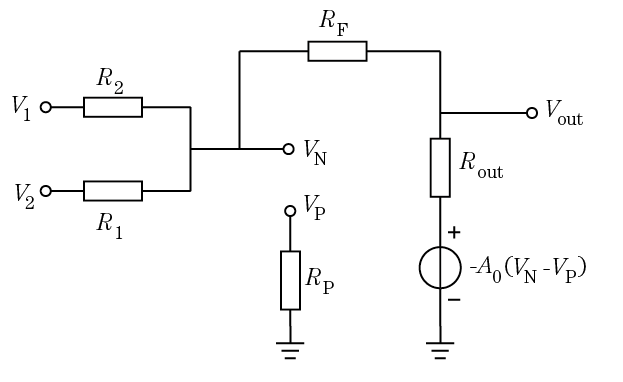
\includegraphics[width=0.415\textwidth]{p8-34-sol.png}
        \caption*{Figure p8-34}
    \end{figure}
        
    $$V_{out} = \frac{(R_1V_1+R_2V_2)\left[1-\frac{R_F(1+A_0)}{R_F+R_{out}}\right]}{R_1 + R_2 + \frac{R_1R_2(1+A_0)}{R_F+R_{out}}}$$
    $$R_{out} \rightarrow +\infty, V_{out} \rightarrow \frac{R_1V_1 + R_2V_2}{R_1+R_2}$$

\paragraph{8.46} \label{8.46}
    Calculate $V_out$ in terms of $V_in$ for the circuit shown in Fig. 8-61.

    \begin{figure}[!htb]
        \centering
        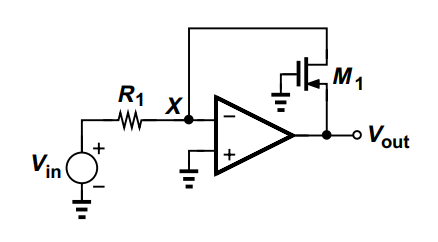
\includegraphics[width=0.292\textwidth]{p8-61.png}
        \caption*{Figure 8-61}
    \end{figure}

\paragraph{解}
    对$M_1$,$V_D = 0$, $I_D = \frac{V_{in}}{R_1}$,又
    $$I_D = \frac{1}{2} \mu_n C_{ox} \frac{W}{L} (-V_{out}-V_{th})^2$$
    $$\therefore V_{out} = \sqrt{\frac{2V_{in}}{R_1\mu_n C_{ox} (\frac{W}{L})}} - V_{th}$$

\paragraph{9.50} \label{9.50}
    Determine the value of $R_P$ in the circuit of Fig. 9-70 such that $I_1 = 2I_{REF}$. With this choice of $R_P$, does $I_1$ change if the threshold voltage of both transistors increases by $\Delta V$?

    \begin{figure}[!htb]
        \centering
        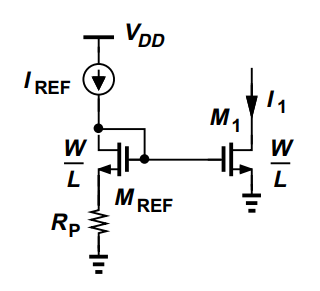
\includegraphics[width=0.213\textwidth]{p9-70.png}
        \caption*{Figure 9-70}
    \end{figure}        

\paragraph{解}
    $M_{REF}$可视为$\under{g_{mREF}}$电阻,源端电压$V_S = I_{REF}R_P$,漏端电压同栅端电压$V_D = V_G=I_{REF}(\under{g_{mREF}}+R_P)$
    \begin{gather*}\left\{\begin{aligned}
        I_{REF} & = \frac{1}{2} \mu_n C_{ox} \frac{W}{L}(I_{REF}\under{g_{mREF}}-V_{th})^2 \\
        I_1 = 2I_{REF} &= \frac{1}{2} \mu_n C_{ox} \frac{W}{L}(I_{REF}(\under{g_{mREF}}+R_P)-V_{th})^2
    \end{aligned}\right.\end{gather*}
    $$\therefore R_P = (\sqrt 2 - 1)(\under{g_{mREF}} - \frac{V_{th}}{I_{REF}})$$
    当确定$R_P$,$V_{th}$增长到$V_{th}' = V_{th}+\Delta V$时,
    $$\frac{I_1}{I_{REF}} = \left(\frac{I_{REF}(\under{g_{mREF}}+R_P)}{I_{REF}\under{g_{mREF}}}\right)^2$$
    \begin{align*}
        \frac{\D I_1}{\D V_{th}}(R_P) & = 2I_{REF} \frac{I_{REF}(\under{g_{mREF}}+R_P)}{I_{REF}\under{g_{mREF}}} \cdot \frac{I_{REF}R_P}{(I_{REF}\under{g_{mREF}}-V_{th})^2} \\
        & = 2\sqrt 2I_{REF}\frac{I_{REF}R_P}{(I_{REF}\under{g_{mREF}}-V_{th})^2} \\
        & = \frac{(4-2\sqrt 2)I_{REF}}{I_{REF}\under{g_{mREF}}-V_{th}}
    \end{align*}
    $$\therefore \Delta I_1 = \frac{(4-2\sqrt 2)I_{REF}}{I_{REF}\under{g_{mREF}}-V_{th}} \Delta V$$

\paragraph{9.52} \label{9.52}
    Calculate $I_{copy}$ in each of the circuits shown in Fig. 9-71. Assume all of the transisitors operate in saturation.

    \begin{figure}[!htb]
        \centering
        \begin{minipage}[t]{0.323\textwidth}
        \centering
        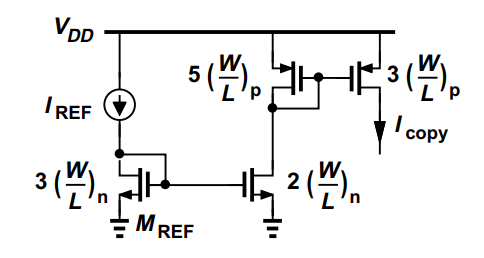
\includegraphics[width=1\textwidth]{p9-71-a.png}
        \caption*{(a)}
        \end{minipage}
        \begin{minipage}[t]{0.394\textwidth}
        \centering
        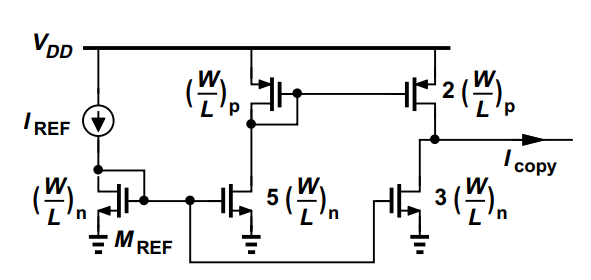
\includegraphics[width=1\textwidth]{p9-71-b.png}
        \caption*{(b)}
        \end{minipage}
        \caption*{Figure 9-71}
    \end{figure}

\paragraph{解} 以下各电流符号中下标表示长宽比所对应的MOS管的电流。

    (a) $I_{2n} = \frac{2}{3}I_{REF}, I_{copy} = \frac{2}{3} \cdot \frac{3}{5} \cdot I_{REF} = \frac{2}{5} I_{REF}$ 

    (b) $I_{5n} = 5I_{REF}, I_{2p} = 10I_{REF}, I_{3p} = 3I_{REF}$
    $$\therefore I_{copy} = 7I_{REF}$$

\end{document} 